% exercise sheet with header on every page for math or close subjects
\documentclass[12pt]{article}
\usepackage[utf8]{inputenc} 
\usepackage{latexsym} 
\usepackage{multicol}
\usepackage{fancyhdr}
\usepackage{amsfonts} 
\usepackage{amsmath}
\usepackage{amssymb}
\usepackage{enumerate}
\usepackage{listings}
\usepackage{graphicx}
\usepackage{pdfpages}

% Shortcuts for bb, frak and cal letters
\newcommand{\E}{\mathbb{E}}
\newcommand{\V}{\mathbb{V}}
\renewcommand{\P}{\mathbb{P}}
\newcommand{\N}{\mathbb{N}}
\newcommand{\R}{\mathbb{R}}
\newcommand{\C}{\mathbb{C}}
\newcommand{\Z}{\mathbb{Z}}
\newcommand{\Pfrak}{\mathfrak{P}}
\newcommand{\Pfrac}{\mathfrak{P}}
\newcommand{\Bfrac}{\mathfrak{P}}
\newcommand{\Bfrak}{\mathfrak{B}}
\newcommand{\Fcal}{\mathcal{F}}
\newcommand{\Ycal}{\mathcal{Y}}
\newcommand{\Bcal}{\mathcal{B}}
\newcommand{\Acal}{\mathcal{A}}

% formating
\topmargin -1.5cm 
\textheight 24cm
\textwidth 16.0 cm 
\oddsidemargin -0.1cm

% Fancy Header on every Page
\pagestyle{fancy}
\lhead{\textbf{Programmierung for Engineers - Exercise 1}}
\rhead{Daniel Schäfer (2549458)\\ Dominik Weber (2548553)\\ Sinah ???? (?????)}
\renewcommand{\headrulewidth}{1.2pt}
\setlength{\headheight}{60pt} 

\begin{document}
\pagenumbering{gobble}
\lstset{language=C}

\section{ Erste Schritte mit dem Arduino Mega}
\begin{enumerate}
    \item 
        ein weiteres \verb!delay! unter der Zeile \verb!digitalWrite(led , LOW);! einfuegen. Siehe zB code aus Aufgabe 1.2 a)
        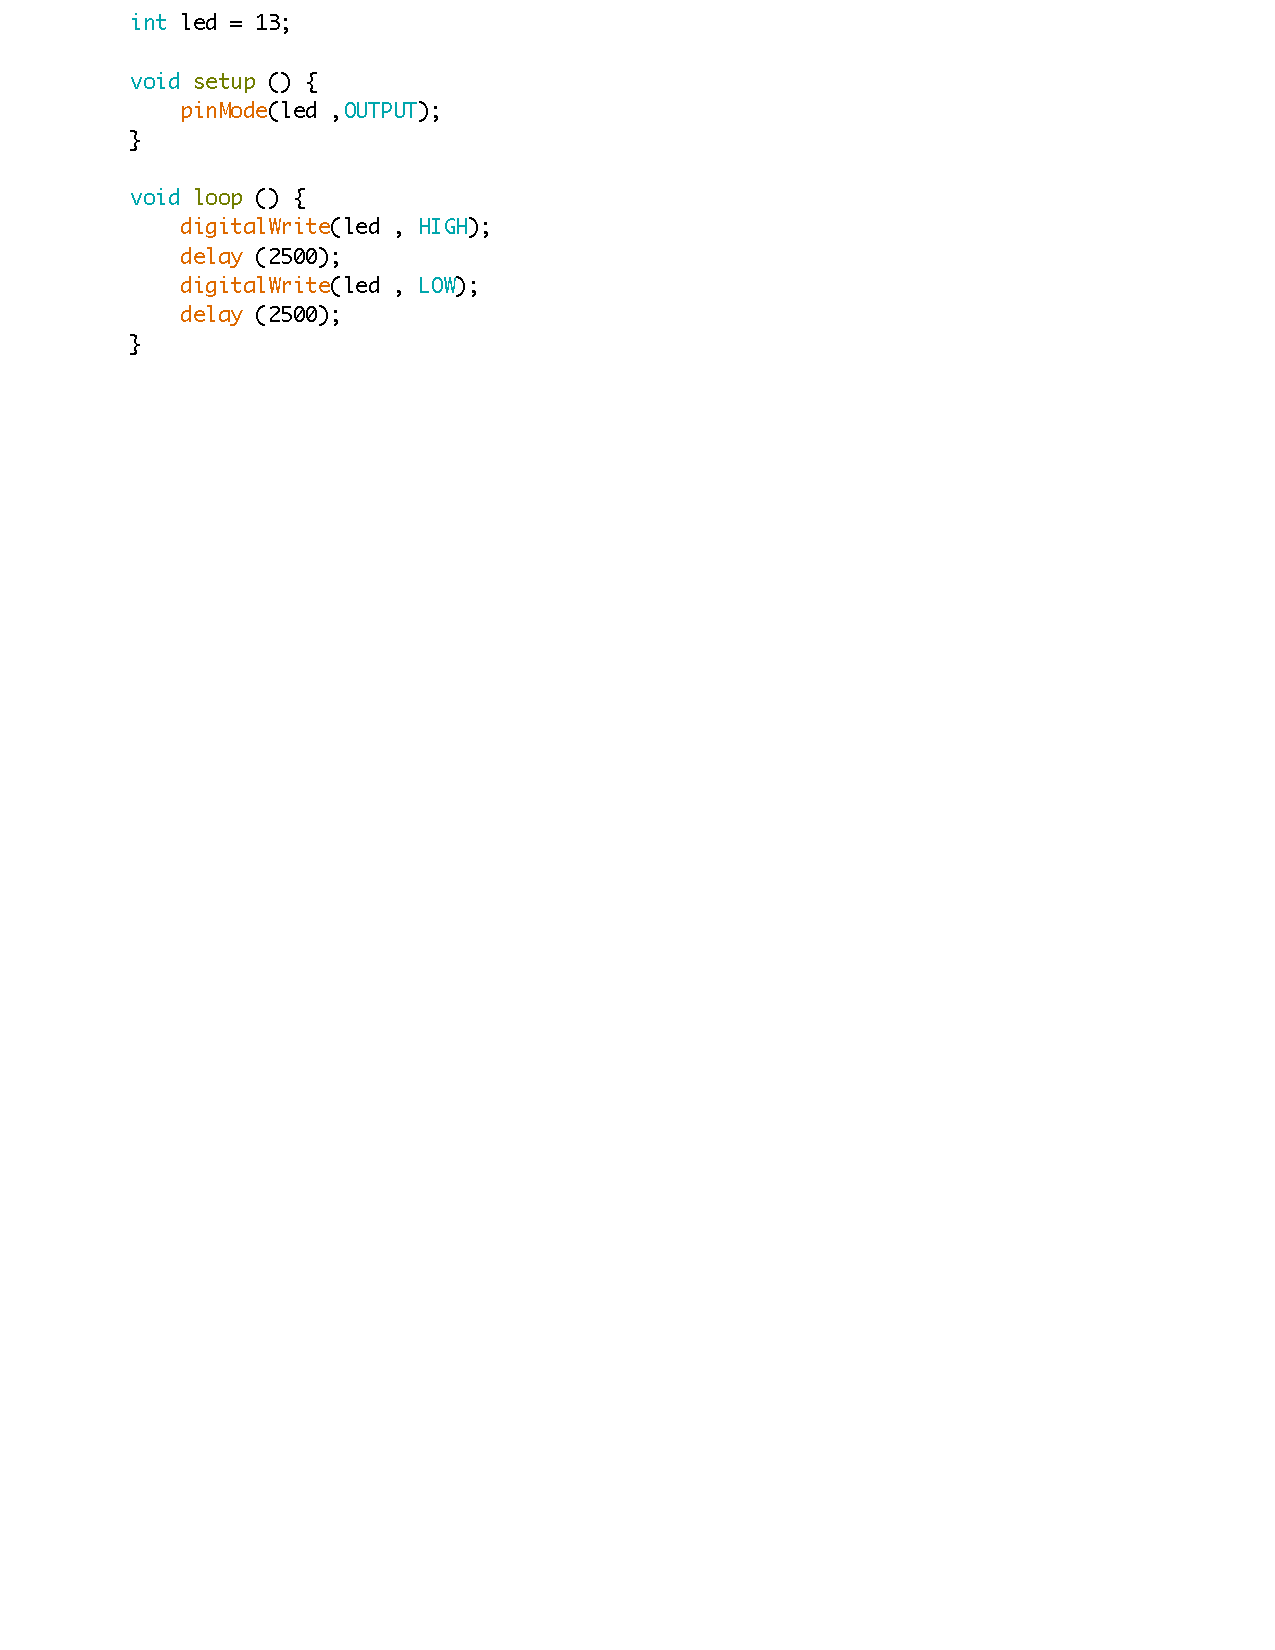
\includepdf[pages=-]{../aufgabe11/aufgabe11.pdf}
    \item
        \begin{enumerate}[a)]
            \item 
                see code on the next page:\\
                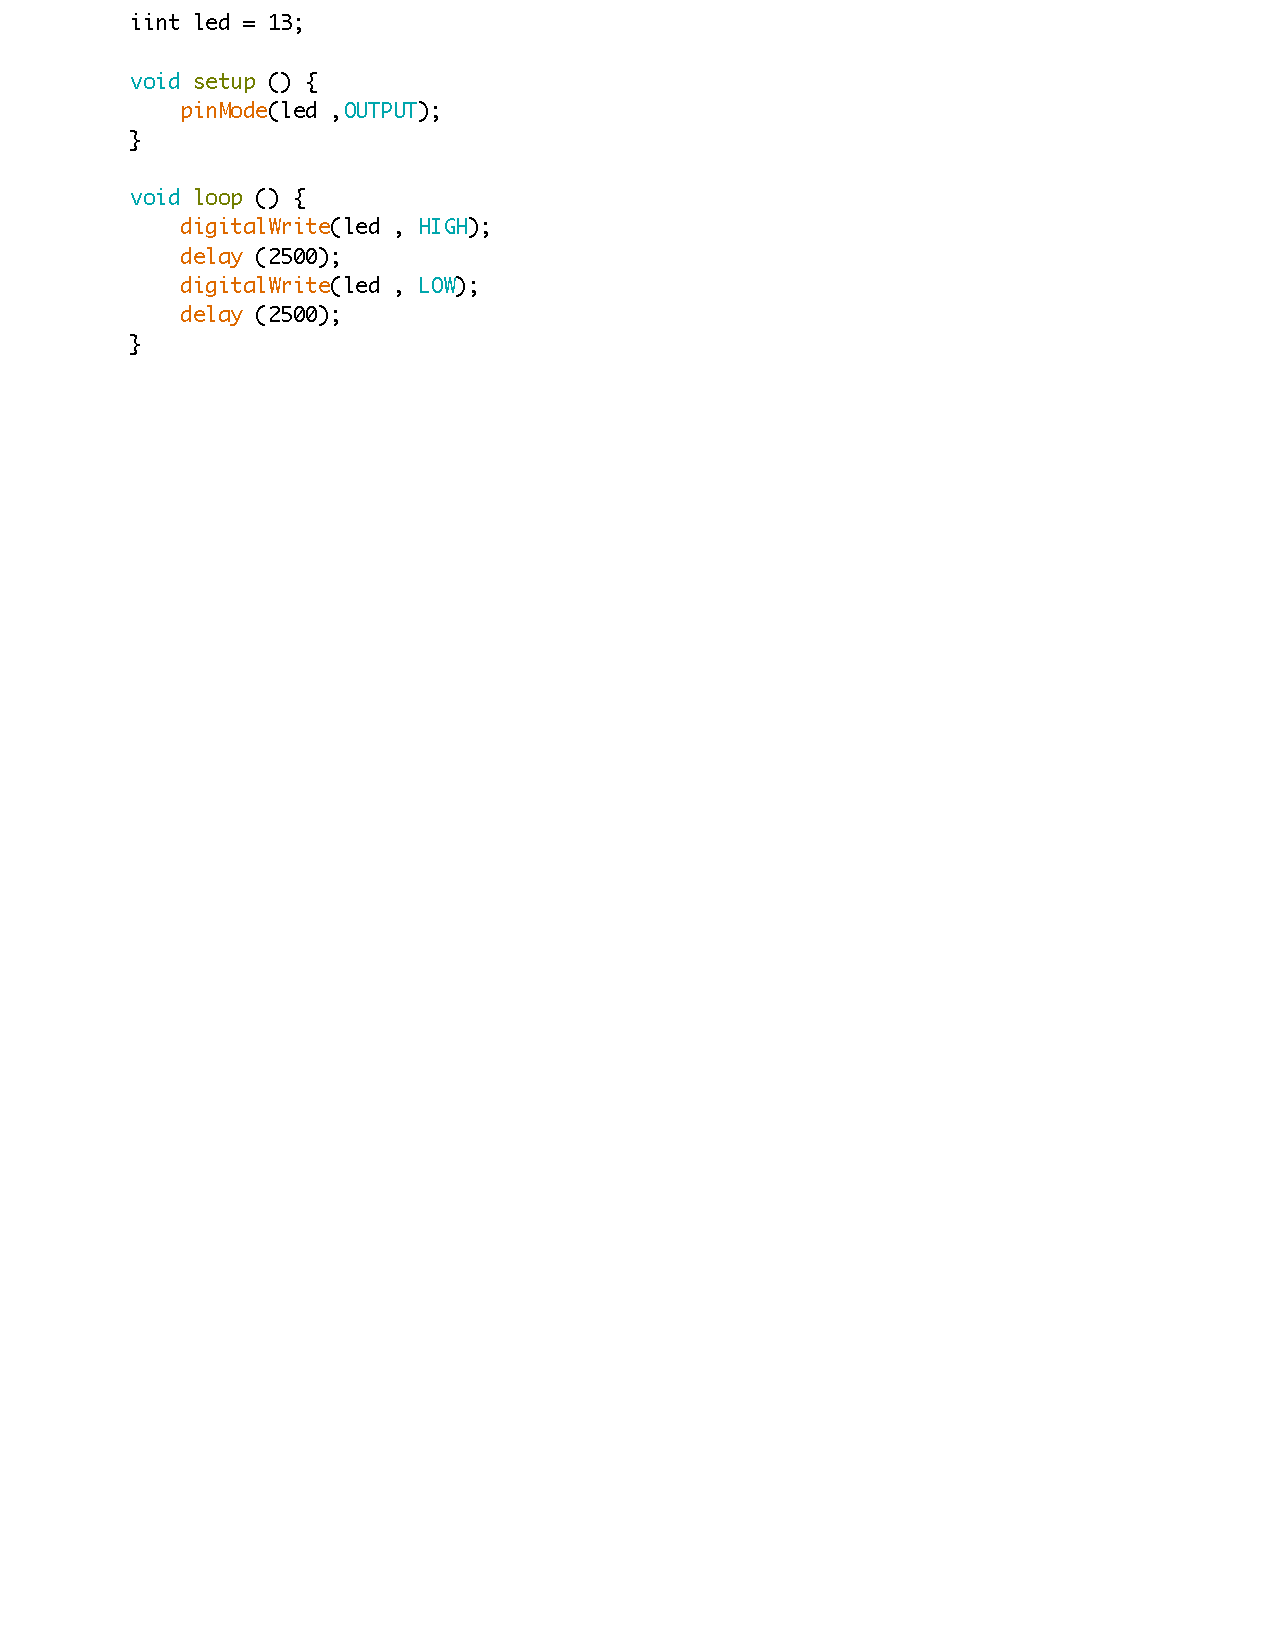
\includepdf[pages=-]{../aufgabe12a/aufgabe12a.pdf}

            \item
                see code on the next page:\\
                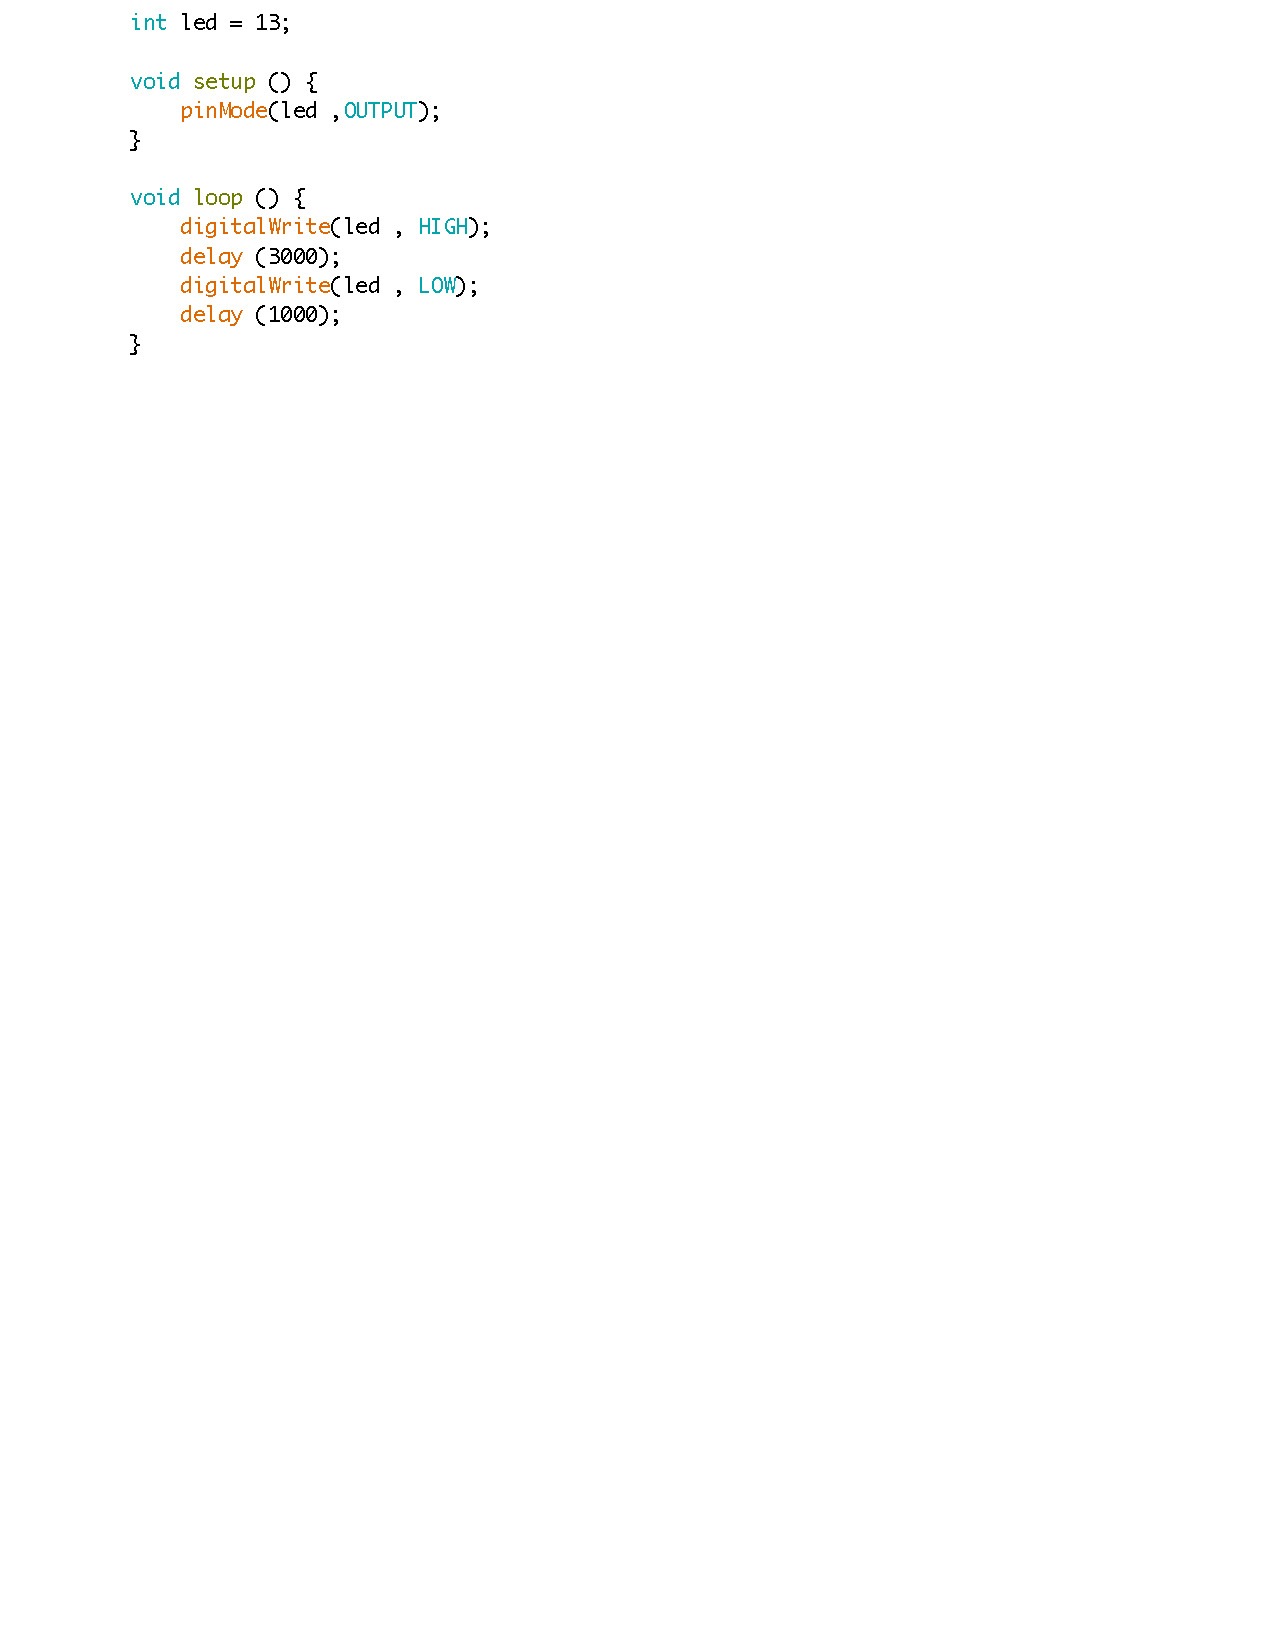
\includepdf[pages=-]{../aufgabe12b/aufgabe12b.pdf}

            \item
                see code on the next page:\\
                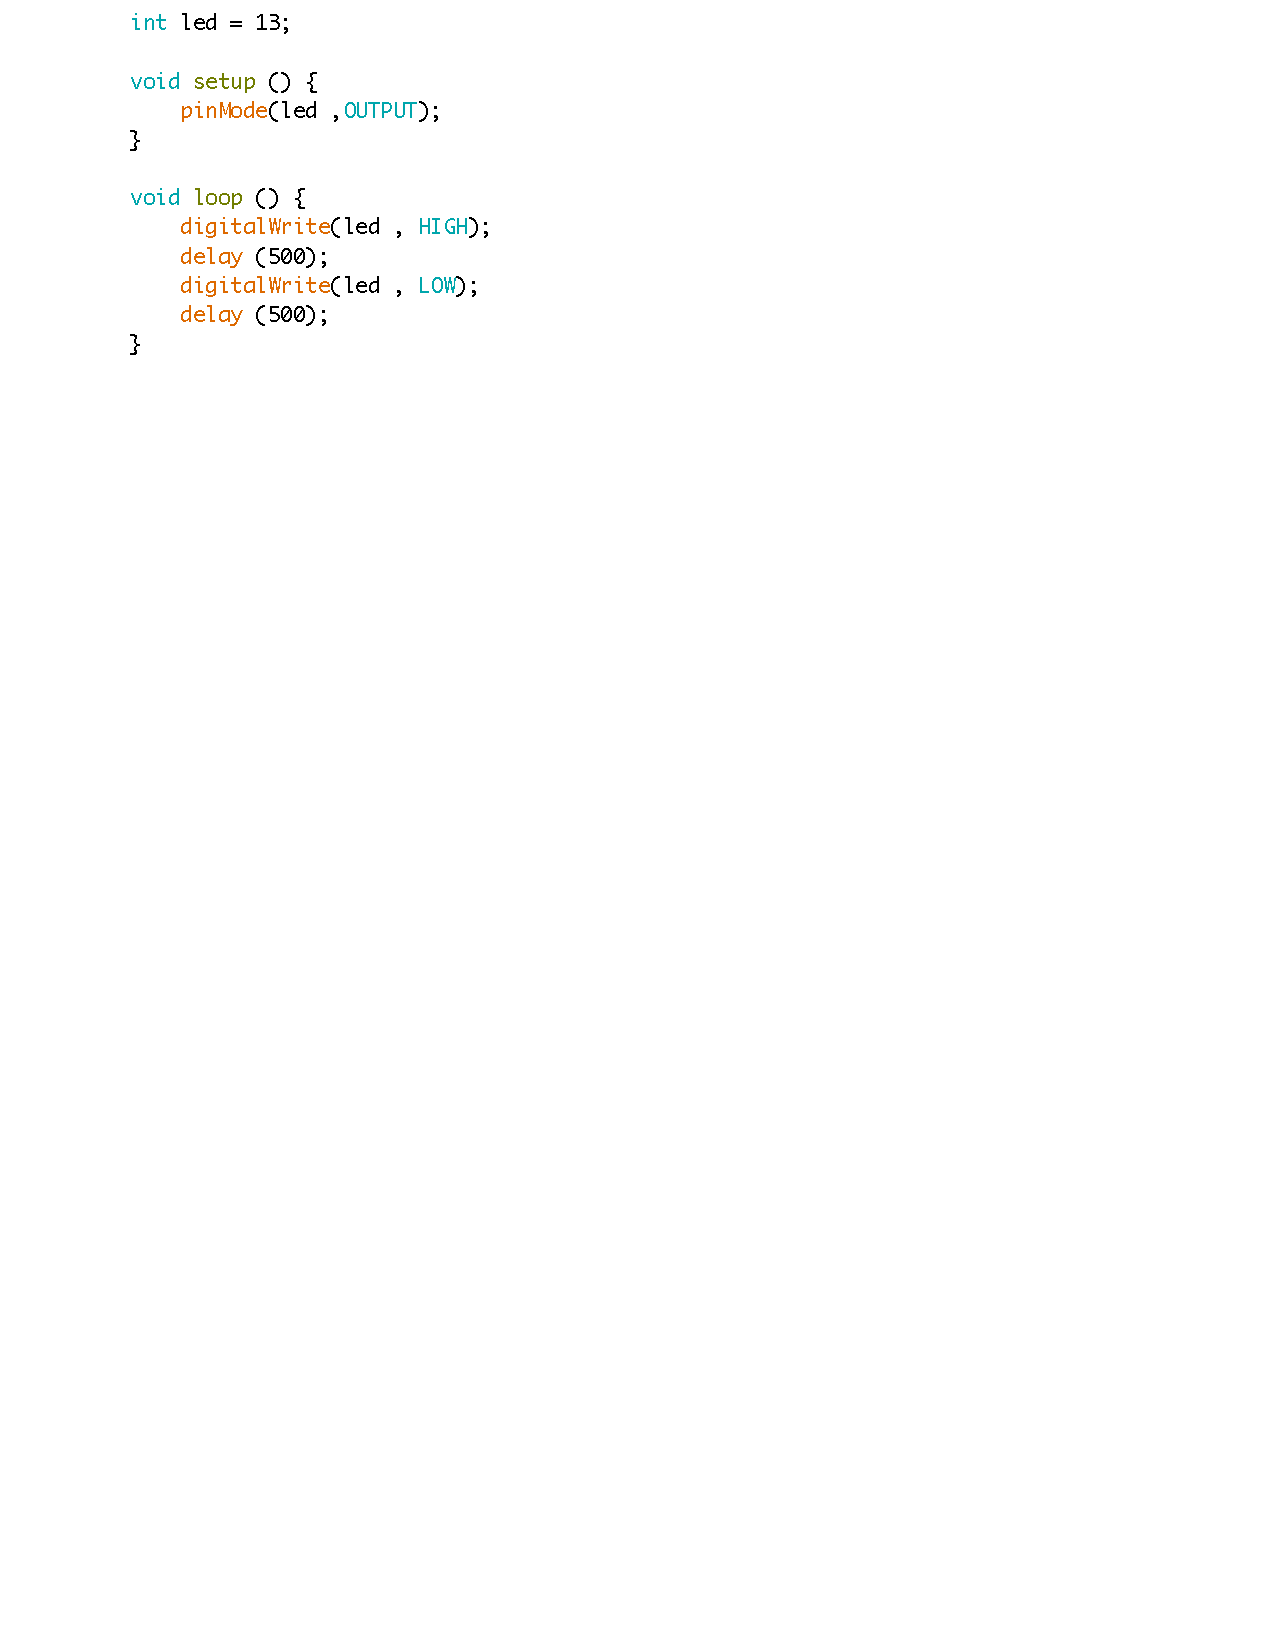
\includepdf[pages=-]{../aufgabe12c/aufgabe12c.pdf}
                
        \end{enumerate}
\end{enumerate}


\section{Morse}

\begin{enumerate}
    \item
        see code on the next page\\
        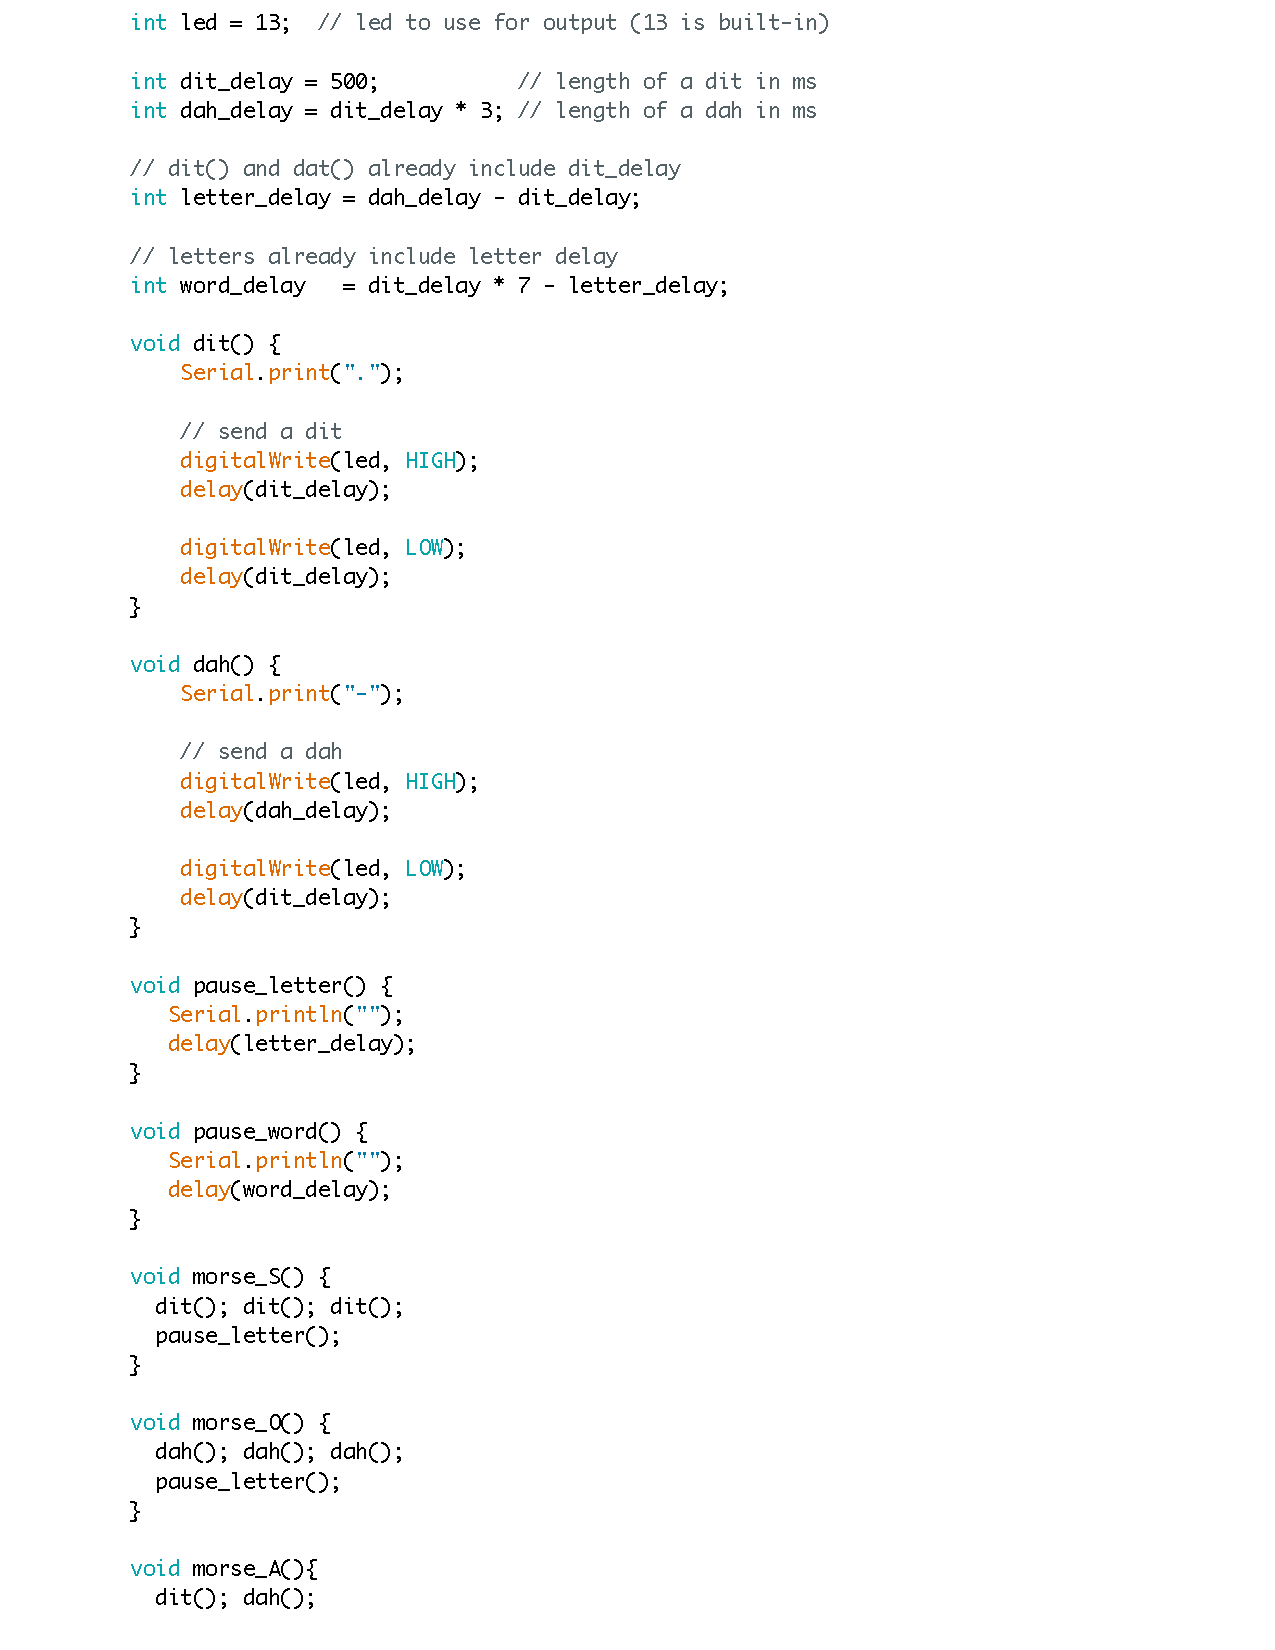
\includepdf[pages=-]{../aufgabe21/aufgabe21.pdf}

    \item
        with the used approach this would be very messy! Essentially you rewrite the approach by using an int argument called \verb!LED_id! to all functions called \verb!morse_A(int LED_id)!, \verb!morse_B(int LED_id)! and so on. Instead of calling \verb! dit()! and \verb!dah()! we would call \verb!dit(int LED_id)! and \verb!dah(int LED_id)!. The functions would look like this:\\

        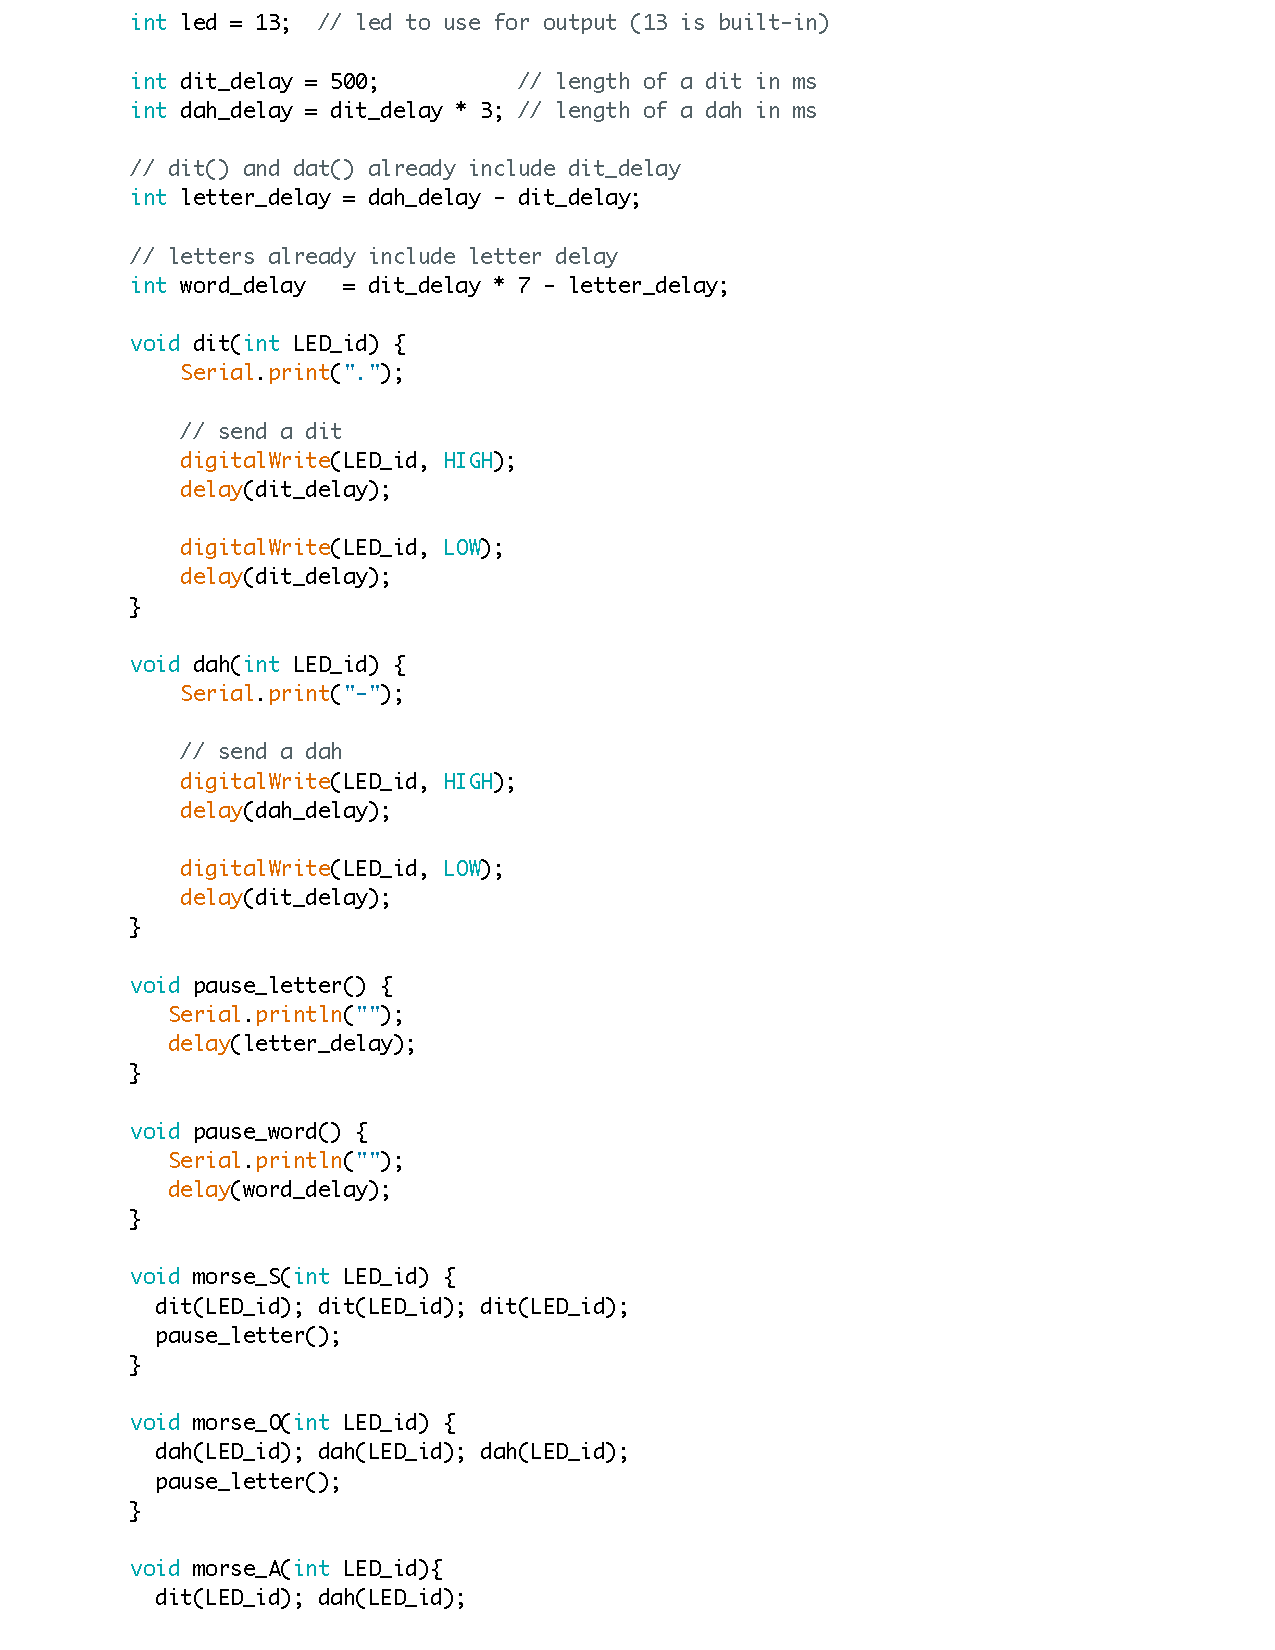
\includepdf[pages=-]{../aufgabe22/aufgabe22.pdf}

        now you can just call the function with the id of the LED you want the letter to appear as shown in the file for this task. You can replace the LED id 12 or 13 with any other LED if you would like!

    \item
        see code on the next page:\\
        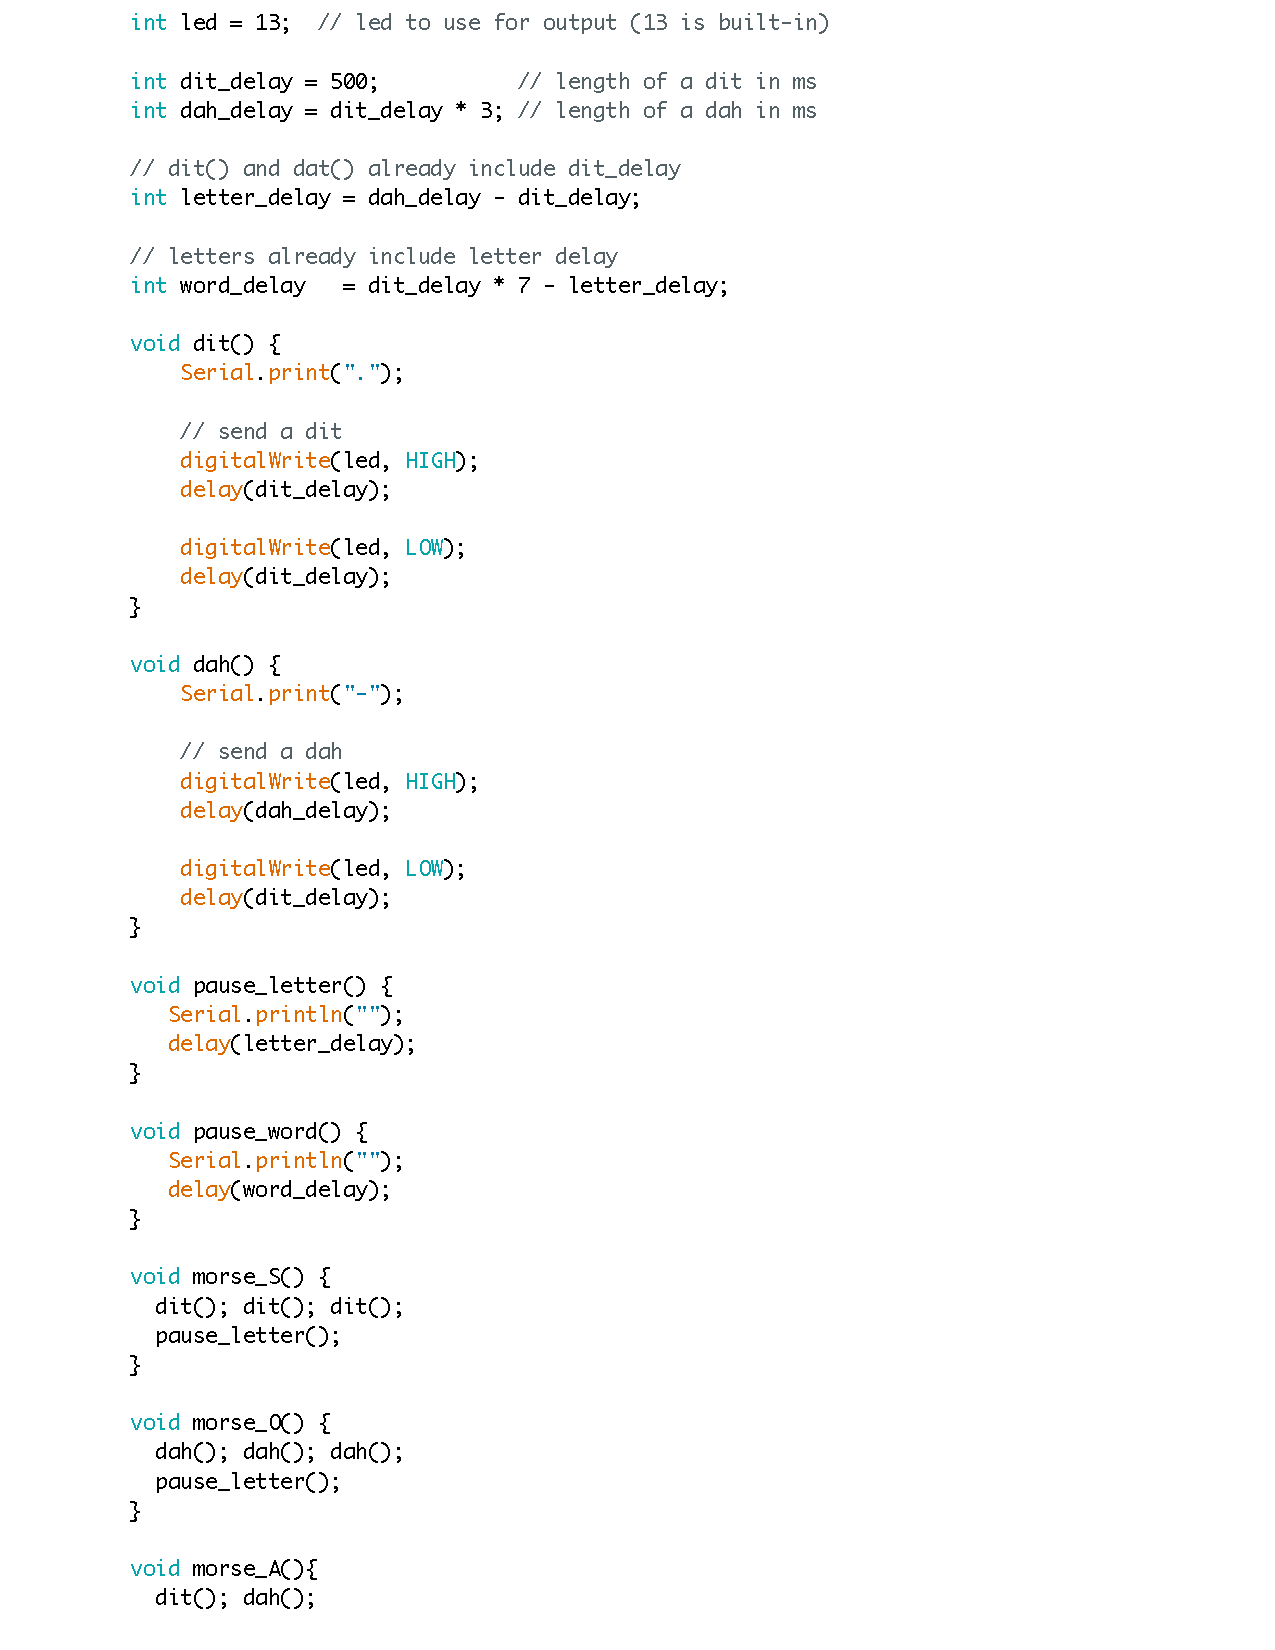
\includepdf[pages=-]{../aufgabe23/aufgabe23.pdf}


\end{enumerate}


\section{Fehlersuche}

yes we get the following error
\begin{verbatim}
Arduino: 1.6.3 (Mac OS X), Board: "Arduino Mega or Mega 2560, ATmega2560 (Mega 2560)"

aufgabe3.ino: In function 'void blink_if_even(int)':
aufgabe3.ino:7:15: error: lvalue required as left operand of assignment
aufgabe3.ino:10:15: error: lvalue required as left operand of assignment
aufgabe3.ino: At global scope:
aufgabe3.ino:15:6: error: variable or field 'setup' declared void
aufgabe3.ino:16:29: error: 'pinmode' was not declared in this scope
aufgabe3.ino:17:5: error: expected '}' before 'pinmode'
aufgabe3.ino:18:1: error: expected declaration before '}' token
Error compiling.

  This report would have more information with
  "Show verbose output during compilation"
  enabled in File > Preferences.

\end{verbatim}
\textbf{Errors explained (and solved)}
\begin{itemize}
    \item 
        ``\verb!lvalue required as left operand of assignment!'' basically means that in line 7 \verb!(n % 2 = 0)! is being interpreted as an assignment (while it should be a comparison), an assignment is only valid if there is an identifier on the left, which is not the case here (its a term). Because we want to compare in this if statement to get a boolean value we have to replace this line with \verb!if (n % 2 == 0)!.

        Exactly the same also applies to line 10

    \item
        ''\verb!variable or field 'setup' declared void!'' shows that our function definition for loop and setup is not understand as such, because the brackets have been forgotten. Change to ''\verb!void setup() {!'' and ''\verb!void loop() {!''

        \item
            ''\verb!error: expected ';' before ...!'' missing semicolon at the end of line 17, 18, 22, 23 and 24.

        \item
            ''\verb!'pinmode' was not declared in this scope!'' shows that the called function does not exist in this function scope. This is caused by a typo, the function ''\verb!pinMode()!'' should be called instead.

        \item
            after fixing all these thrown errors the programm is still not working as intended for multiple reasons. The next problem we should fix is the bracketing of the if statements around the digitalWrite calls. It should be done like this:\\

            \newpage
\begin{verbatim}

if (n % 2 == 0) {// even
    digitalWrite(led_red , HIGH);
    digitalWrite(led_green , LOW);
}
if (n % 2 == 1) {// odd
    digitalWrite(led_red , LOW);
    digitalWrite(led_green , HIGH);
}

\end{verbatim}

Corrected File:\\
        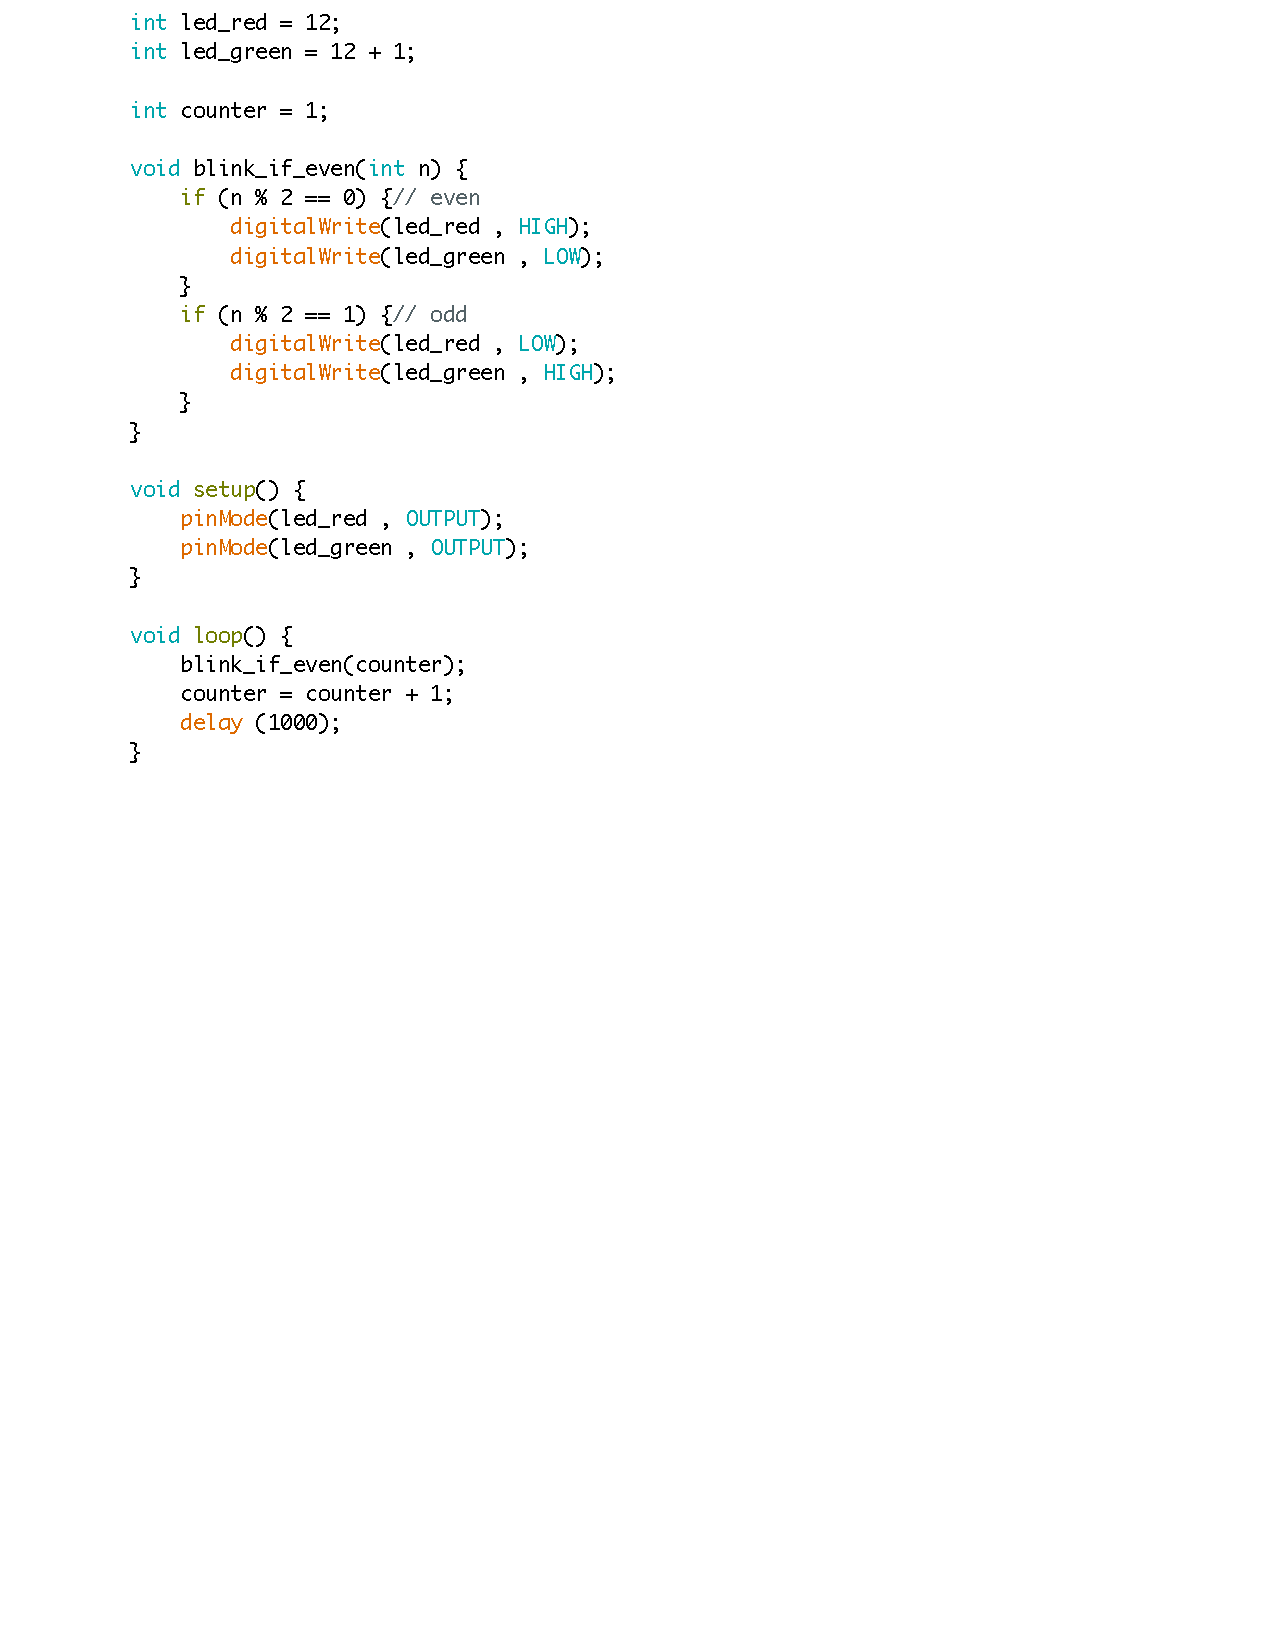
\includepdf[pages=-]{../aufgabe31/aufgabe31.pdf}


\end{itemize}

\textbf{Eleganter:}\\
A much quicker and more elegant option would be to do it like this:
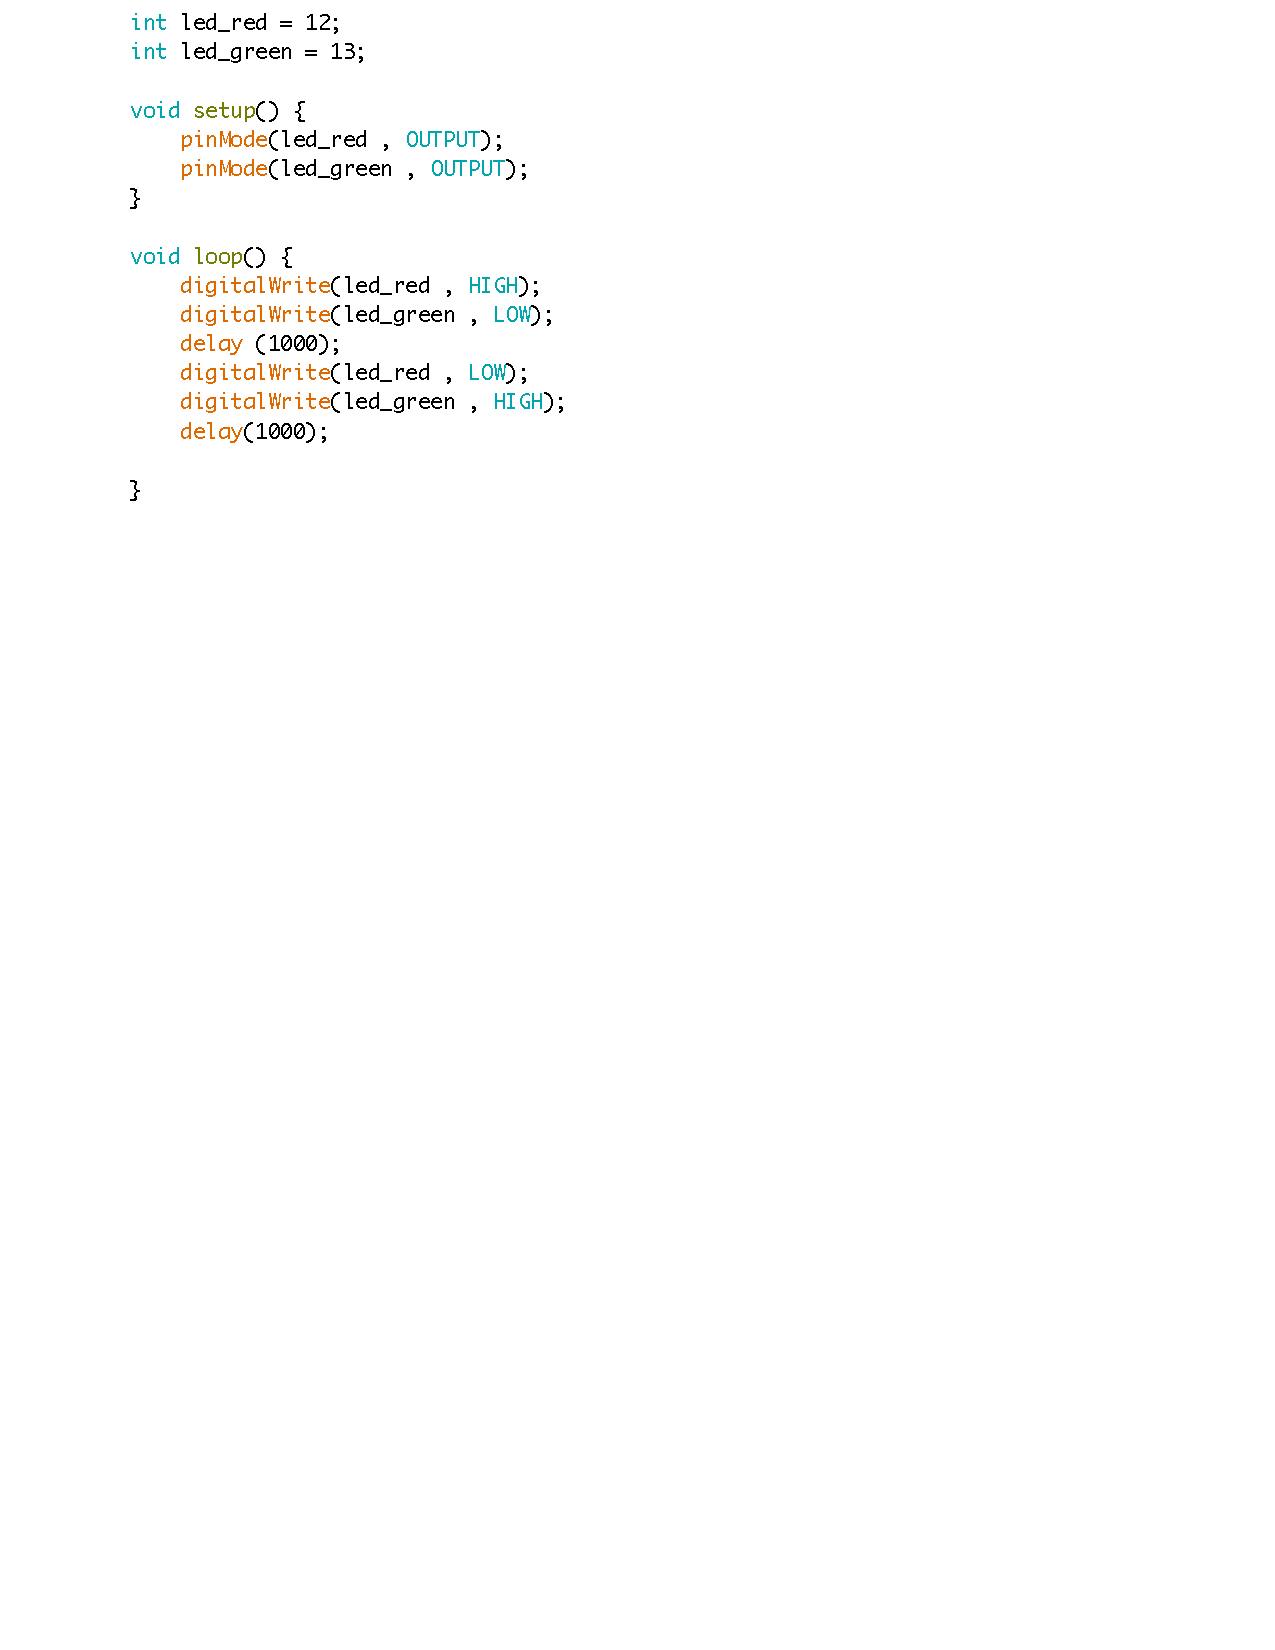
\includepdf[pages=-]{../aufgabe32/aufgabe32.pdf}


\end{document}
